\documentclass[conference]{IEEEtran}
\IEEEoverridecommandlockouts

\usepackage{listings}
\usepackage{hyperref}
\usepackage{amsmath}
\usepackage{graphicx}
\usepackage{tabularx}
\def\BibTeX{{\rm B\kern-.05em{\sc i\kern-.025em b}\kern-.08em
    T\kern-.1667em\lower.7ex\hbox{E}\kern-.125emX}}
\begin{document}
\title{Implementation of Concurrent Hash Tables in Java}

\author{\IEEEauthorblockN{ Shawn Guydeene}
\and
\IEEEauthorblockN{ Dalton Kajander}
\and
\IEEEauthorblockN{ Blake Celestian}
}

\maketitle

\begin{abstract}
    Concurrent programming is using multiple processes at the same time, often reducing total time waiting for operations to complete. A concurrent hash table is a hash table that utilizes concurrent programming in order to reduce the time it takes to do multiple operations, such as the add(), search(), and remove() methods hash tables utilize. It does this by doing different operations at the same time instead of one after another, waiting for the previous to finish before the next can even start. This report is about attempting to create our own concurrent hash table in the Java language instead of using Java’s own HashTable class. We will be achieving this by using function keywords like “synchronized” and manually locking and unlocking, experimenting will both options. We will show evidence of reduced time by running the same commands on an unthreaded custom HashTable and on a custom concurrent HashTable.
\end{abstract}

\begin{IEEEkeywords}
Concurrent Programming, Hash-table representations
\end{IEEEkeywords}

\section{Introduction}
The problem that our group chose to tackle, is how one would parallelize a hash table, and see how much of a performance increase,
if any would arise from such an implementation. This paper seeks to explain the how hash tables function as a data structure, previous
attempts at parallelizing them, our group's attempt at creating a concurrent hash table, and experimental data collected showing the
effects of parallelizing on runtime for the program.

\section{Research}
\subsection{What are Hash Tables?}
Hash tables are a data structure that utilizes an associative array, which is a structure that associates keys to specific values, in order to store data. The way
in which a hash table uses these keys, is by entering them into a hash function. The hash function will then compute the array index in which
the value associated with the key will be stored. The hash function is naturally the most important portion of the hash table's construction.
The most commonly used hashing methods uses some variation of modular hashing. Modular hashing works as follows: assuming there is an array of size
$M$, where $M$ is prime, then for any positive integer key $k$, compute $k \mod{M}$. 

Modular hashing is expandable to accepting more than just integer as keys. A common data type used as a key for hash tables would be strings.
In order to accomplish this, one would simply have to treat the string as though it were a large integer. This concept of converting data types into
integers is commonly used as it is much simpler than creating a custom hashing function. A well made hash function will have three main requirements:
deterministic - equivalent keys will always produce the same hash value, computationally efficient, and allows for keys to be uniformly distributed.
Deterministic is only one of those requirements that is absolutely necessary for any hash function, as it what allows users to search hash tables
for a specific key-value pairing [1].

There is of course, one issue with the hash function: since the hash table is not an array of infinite size, there is guaranteed to be instances where
two distinct keys map to the same index when using the hash function. In order to resolve this, several techniques have been developed: linear probing,
quadratic probing, double hashing, separate chaining or buckets. The basic concept for linear probing is that if the current key-value attempting to be
entered into the hash table collides at position $i$, then attempt to place it at $i+1$. If it collides again, keep increasing the index by $1$ until
it comes across an index in the hash table array that has not been used yet, ending at $i+n$ where $n$ is the number of collisions. Quadratic probing is
similar to linear probing, except instead of ending up at $i+n$, the value will be stored at index $i+n^2$, where $n$ is the number of collisions.
Double hashing, also known as rehashing, involves hashing the key a second time, with a different hash function. That result is taken, and then used as
the step size for a process similar to the previous two methods, resulting in the value being place at index $i+jn$, where $n$ is the number of collisions,
and $j$ is the result of the second hash function. These methods, known as open addressing, work, but as the hash table begins to fill up, they result in the 
add() operation taking more time to complete due to collisions. Separate chaining, on the other hand, works by having each index of the array be a linked list. 
Whenever a value maps to that index, it will be added into list, which avoids the issue that open addressing presents. Buckets is a similar method to 
separate chaining, using an array instead of a linked list. While separate chaining and buckets fix the issues with open addressing, they present more
of their own, namely that there exist the possibility that a large majority of keys will map to the same index, which leads to a large amount of time
being used searching the array or list at that index for the specified key's value [2].

\subsection{What is Concurrency?}
Now given what a hash table is, this paper will look at what exactly it means for a computer program to be concurrent. Concurrency means that multiple computations
will be occurring at the same time. This has become increasing more important, with the clock speed of processors no longer increasing, it results in 
manufacturers adding more cores to chips, meaning splitting up computation among those chips is the only way to make it faster. Concurrent programming
has two common models: shared memory models and message passing models. This paper will only look at shared memory models as the implementation for
a concurrent hash table will utilize a shared memory model. A shared memory model works by having concurrent processors read and write objects into the
memory that they share [3].

\subsection{Challenges of Concurrency}
The largest challenge of creating any concurrent program is the concept of thread safety. For a data structure or algorithm to be consider threadsafe, it 
must behave correctly when multiple threads are using it, without additional instructions from the function calling it. There are many strategies to utilize for
creating a threadsafe data structure. One such strategy is known as \emph{confinement}, which avoids the issue of threads reading and writing to the same
memory location because all the data is confined to a single thread, and the other threads do not have the ability to read or write to memory directly.
Another strategy is \emph{immutability}, which means that the information which the threads share will be immutable, meaning they are unable to be altered by
the threads. Other than those two, there is also the strategy of utilizing \emph{threadsafe data types}. Naturally utilizing data types that are already designed
to be threadsafe helps when creating threadsafe algorithms and data structures because these data types are designed to not fail when multiple threads are being used
[4]. There is one final strategy for desgining a threadsafe program, and that is to synchronized the threads so that they do not attempt to read or write to the same
memory location at the same time. The most common way to implement thread synchronization in shared memory models is the use of locks. The way locks works is by taking
the part of the program that accesses the data, and creating a "lock" around it. What this lock does is prevent multiple threads from being with in the "locked" region
of the code. If a thread will attempt to enter the "locked" region, while another thread is already inside of it, the other thread will be a frozen 
until the lock is removed and the thread will be able to access the region, reinitiating the lock again to prevent another thread from entering. Now that no other threads
can enter the "locked" region, the thread inside of it is able to alter the memory location without having any other threads attempting to access it at the same time.

\section{Algorithms}
\subsection{Basic Hashtable}
\begin{lstlisting}[language={Java},caption=Source code for the course-grain put() method.,captionpos=b,breaklines=true,frame=single]
public synchronized boolean put(int item) {
    // If capacity if full, do not add
    if (capacity >= ARR_SIZE)
        return false;

    // Get key
    int key = hash(item);

    // Check if first try addition
    if (table[key] == null) {
        table[key] = item;
        cleans[key] = false;
    }
    // Otherwise, quadratically probe for empty indices
    else {
        int i = 1;
        int new_key = (key + i) % ARR_SIZE;
        while (table[new_key] != null) {
            i++;
            new_key = (new_key + i) % ARR_SIZE;
        }
        table[new_key] = item;
        cleans[new_key] = false;
    }

    // Increase capacity
    capacity++;
    return true;
}
\end{lstlisting}
\section{Experimental Results}
We began by testing how the standard hash table will performed when run sequentially, and then when multithreaded. 
After those tests, we created a locking hash table and proceeded to run tests on that version. 
After both of those tests, we deicded it would be a good idea to test our hash tables to Java's native concurrent hash map, the closest thing to a concurrent hash table Java has to offer natively.
Our measurement for testing was timing how long each hash table takes to add a specific amount of numbers, make sure each one was added, remove all those numbers, and then make sure each was removed. 
We recorded all the measurements into a CSV file and used a Python program to analyze the numbers, using Pandas to do the math and Matplotlib and Seaborn to visualize the data gathered. 
We were able to gather a plentiful amount of information regarding each hash table and the time it takes to do these processes. 
The data we gathered includes total time taken, the CPU used, the amount of tests, the time it took to do each test for each hash table, the average, low, and high times, and the standard deviation. All times recorded are in millisecconds. 
\begin{figure}[htbp]
    \centerline{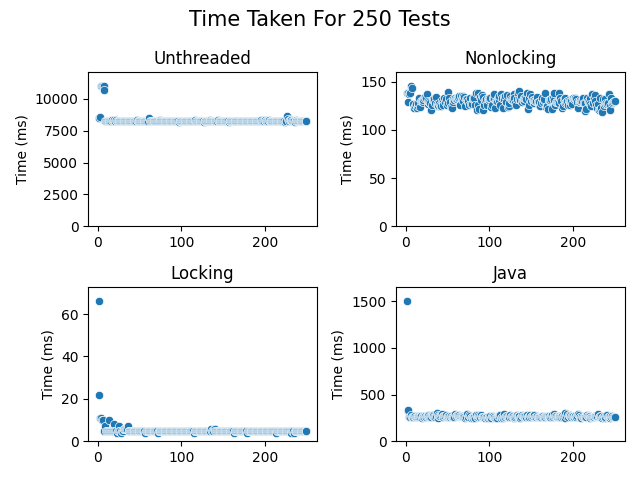
\includegraphics[width=90mm,scale=1]{250trials.png}}
    \caption{Graphs of each test for each hash table. The x-axis is the test number, the y-axis is the time in ms the test took. }
    \label{fig}
\end{figure}

\begin{table}[htbp]
    \caption{Experimental Results}
    \begin{center}
    \begin{tabularx}{\columnwidth}{|X|X|X|X|X|}
    \hline
    \textbf{Data}&\multicolumn{4}{|c|}{\textbf{Hash Table Version}} \\
    \cline{2-5} 
    \textbf{Calculation} & \textbf{\textit{Nonlocking}}& \textbf{\textit{Threaded}}& \textbf{\textit{Locked Threaded}}& \textbf{\textit{Java}} \\
    \hline
    \textbf{Average}& 8,135 ms& 130 ms&  5 ms& 272 ms\\
    \hline
    \textbf{High}& 10,978 ms& 145 ms&  66 ms& 1,499 ms\\
    \hline
    \textbf{Low}& 8164 ms& 118 ms&  4 ms& 247 ms\\
    \hline
    \textbf{Deviation}& 376.3 ms& 4.5 ms&  4.1 ms& 78.7 ms\\
    \hline
    \textbf{Total time}&\multicolumn{4}{|c|}{\textbf{2,180,629 ms}} \\
    \hline
    \multicolumn{5}{l}{Threaded is Nonlocking but concurrently tested instead}
    \end{tabularx}
    \label{tab1}
    \end{center}
\end{table}




\begin{thebibliography}{00}
\bibitem{b1} R. Sedgewick and K. Wayne. ``Hash Tables." princeton.edu. \\https://algs4.cs.princeton.edu/34hash/ (accessed Mar. 13, 2022).
\bibitem{b2} S. Mitra. ``Hashing." utexas.edu. https://www.cs.utexas.edu/~mitra/\\csSpring2017/cs313/lectures/hash.html (accessed Mar. 13, 2022).
\bibitem{b3} S. Amarasinghe, A. Chlipala, S. Devadas, M. Ernst, M. Goldman, J. Guttag, D. Jackson, R. Miller, M. Rinard, and A. Solar-Lezama. ``Reading 17: Concurrency"
mit.edu. https://web.mit.edu/6.005/\\www/fa14/classes/17-concurrency/ (accessed Mar. 14, 2022).
\bibitem{b3} S. Amarasinghe, A. Chlipala, S. Devadas, M. Ernst, M. Goldman, J. Guttag, D. Jackson, R. Miller, M. Rinard, and A. Solar-Lezama. ``Reading 18: Thread Safety"
mit.edu. http://web.mit.edu/6.005/\\www/fa14/classes/18-thread-safety/ (accessed Apr. 20, 2022).
\bibitem{b3} S. Amarasinghe, A. Chlipala, S. Devadas, M. Ernst, M. Goldman, J. Guttag, D. Jackson, R. Miller, M. Rinard, and A. Solar-Lezama. ``Reading 20: Queues \& Locks"
mit.edu. http://web.mit.edu/6.005/\\www/fa14/classes/20-queues-locks/(accessed Apr. 20, 2022).
\end{thebibliography}
\end{document}